\documentclass[fontset=windows]{article}
\usepackage[margin=1in]{geometry}%设置边距，符合Word设定
\usepackage{ctex}
\usepackage{setspace}
\usepackage{lipsum}
\usepackage{amsmath}
\usepackage{graphicx}%插入图片
\usepackage{tikz}
\usetikzlibrary{arrows.meta,decorations.markings,patterns,calc}

\usepackage{xcolor}
\graphicspath{{Figures/}}%文章所用图片在当前目录下的 Figures目录

\usepackage{hyperref} % 对目录生成链接，注：该宏包可能与其他宏包冲突，故放在所有引用的宏包之后
\hypersetup{colorlinks = true,  % 将链接文字带颜色
	bookmarksopen = true, % 展开书签
	bookmarksnumbered = true, % 书签带章节编号
	pdftitle = This is a testfile for vscode, % 标题
	pdfauthor =Ali-loner} % 作者
\bibliographystyle{plain}% 参考文献引用格式
\newcommand{\upcite}[1]{\textsuperscript{\cite{#1}}}

\renewcommand{\contentsname}{\centerline{Contents}} %经过设置word格式后，将目录标题居中


\title{\heiti\zihao{2} This is a testfile for vscode}
\author{\songti Ali-loner}
\date{2020.08.02}


\begin{document}
	\maketitle
	\thispagestyle{empty}

\begin{abstract}
	\lipsum[2]
\end{abstract}

\tableofcontents

\section{This is a section}
Hello world! Hello Ali! As shown in figure \ref{1}
\begin{figure}[htbp]
	\centering
	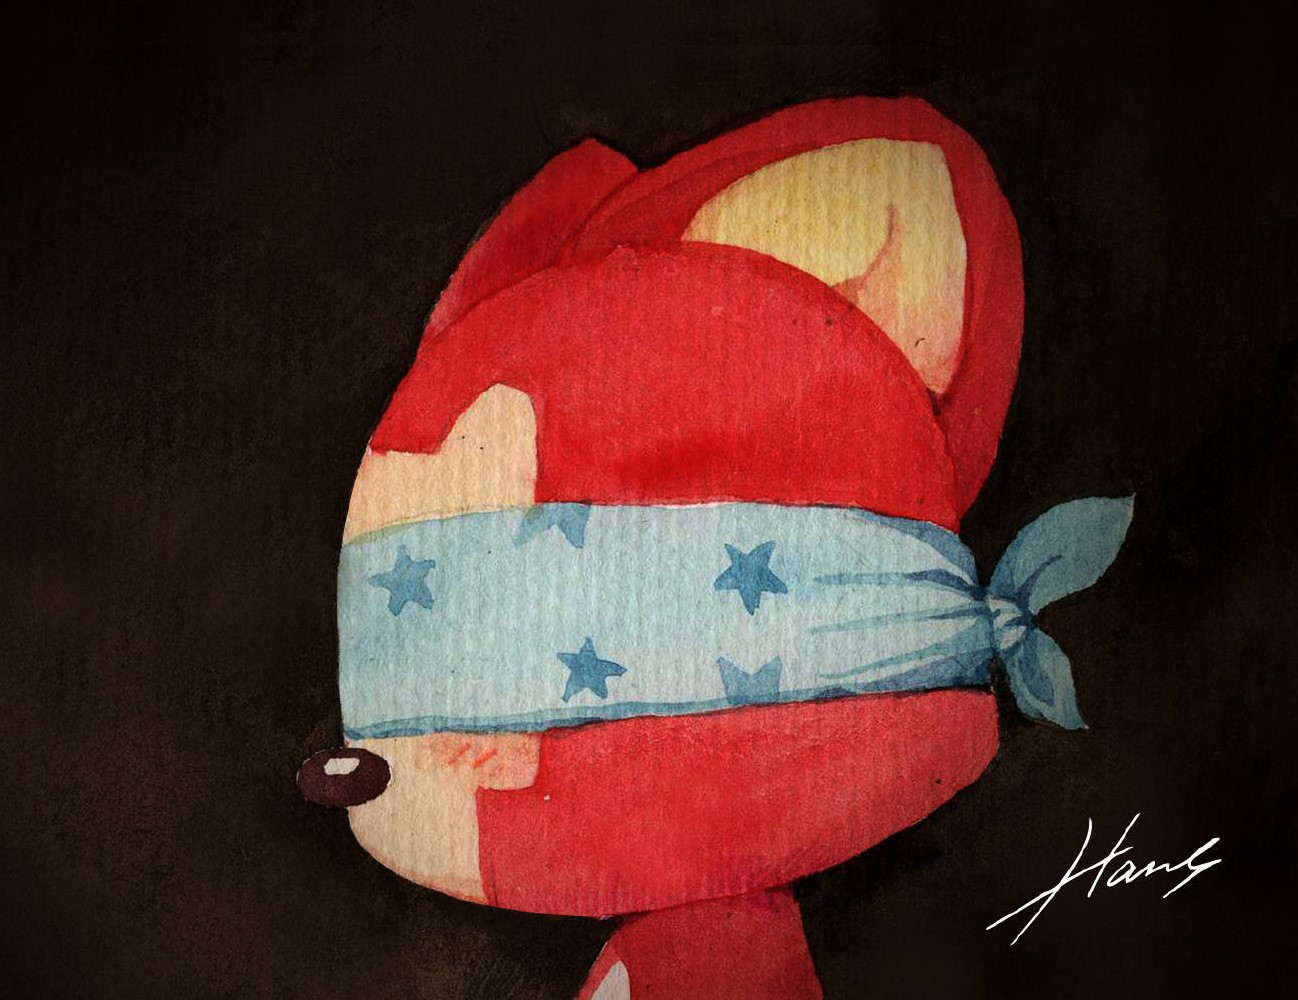
\includegraphics[scale=0.2]{Ali.jpg}
	\caption{this is Ali}
	\label{1}
\end{figure}





\subsubsection{improvement of the Strategies on Curved Roads}
在自行车个人计时赛中，弯道往往构成决定性约束。与直线路段不同，骑手在弯道中不仅需要提供沿行进方向的驱动力（或制动力），还必须同时产生足够的横向力以维持转向运动。由于轮胎与路面之间的摩擦力存在物理极限，骑手在弯道中的受力分配直接制约其可行速度与加速策略。

传统配速模型通常假设骑手在弯道中以最大安全速度匀速通过，即将弯道简化为纯速度约束。
然而，该处理忽略了一个重要事实：在摩擦力允许的范围内，骑手可以通过合理分配驱动力，在弯道中实现加速或减速，从而获得更优的整体配速方案。

设自行车与骑手的总质量为 $m$，重力加速度为 $g$，轮胎与路面的摩擦系数为 $\mu$，则轮胎所能提供的最大摩擦力为$
f_{\max} = \mu m g .$
在弯道行驶过程中，轮胎摩擦力可分解为两个相互正交的分量：
\begin{itemize}
    \item 沿行进方向的切向摩擦力 $F_x$，用于驱动或制动；
    \item 垂直于行进方向的横向摩擦力 $F_c$，用于提供向心力。
\end{itemize}
根据摩擦圆（Friction Circle）约束，总摩擦力的合力不得超过摩擦极限，因此有
\begin{equation}
\sqrt{F_x^2 + F_c^2} \leq \mu m g .
\label{eq:friction_circle}
\end{equation}
设弯道曲率半径为 $R$，骑手以速度 $v$ 行驶时所需的向心加速度为
$
a_c = \frac{v^2}{R},
$
对应的向心力为$F_c = m \frac{v^2}{R}.$
将上述关系代入式 \eqref{eq:friction_circle}，可得
\begin{equation}
F_x^2 + \left( m \frac{v^2}{R} \right)^2 \leq (\mu m g)^2 .
\end{equation}
整理后得到在给定切向力 $F_x$ 条件下的速度上界：
\begin{equation}
v \leq 
\sqrt[4]{\left( \mu g R \right)^2 - \left( \frac{F_x R}{m} \right)^2 }.
\label{eq:vmax_corner}
\end{equation}

该约束表明，骑手在弯道中施加的驱动力或制动力越大，可用于提供向心力的摩擦裕度越小，从而限制最大可行速度。

为了得到通过该弯道的最短时间，我们将赛道沿弧长方向离散为 $N$ 个微小路段，每段长度为 $ds$，第 $i$ 段对应的曲率半径为 $R_i$。定义第 $i$ 段的速度与切向力分别为 $v_i$ 与 $F_{i,x}$，则每个离散路段均需满足
\begin{equation}
v_i \leq 
\sqrt[4]{\left( \mu g R_i \right)^2 - \left( \frac{F_{i,x} R_i}{m} \right)^2 }.
\end{equation}
相邻路段之间的速度变化由切向加速度 $a_x$ 决定，满足一维运动学关系
$
v_{i+1}^2 - v_i^2 = 2 a_x ds.
\label{eq:kinematics}
$然而$a_x$并非自由取值。
一方面，轮胎总摩擦力必须位于摩擦圆内,另一方面
考虑骑手最大可输出功率限制
$P_{\text{out}} \leq P_{\max}.$
最终以全程用时最短为目标，得到目标函数：
\begin{equation}
T = \sum_{i=1}^{N} \frac{ds}{v_i}.
\end{equation}
\subsection{11}
为了验证我们所建弯道配速优化模型的合理性与优越性，
我们以日本的56号赛段的弯道为测试对象，
采用改进后的弯道的动力学与运动学模型，使用matlab的fmincon优化器进行求解，
得到结果\autoref{1}。
\begin{figure}[htbp]
	\centering
	
\includegraphics[width=1\textwidth]{Figures/image.png}
	\caption{效果对比}
	\label{1}
\end{figure}
结果表明，传统模型在弯道处采用最大安全速度匀速通过策略，
其弯道速度受向心力单独约束，计算得到极限速度约为$5.8m/s$
相比之下，本文所建模型允许在满足摩擦圆约束的前提下，
在弯道中合理分配切向力与向心力，从而实现弯道内的非匀速运动。
优化模型在弯道处极限的速度可提升至$9.64m/s$,

功率输出曲线进一步揭示了两种模型在弯道策略上的本质差异。
在传统模型中，骑手在弯道内保持匀速行驶，对应切向力接近零，
功率输出显著下降，导致弯道阶段成为“纯损失时间段”。
而在优化模型中，骑手在入弯前主动减速并降低功率输出，在弯道核心区间内维持中等功率水平，
同时严格受最大功率约束
$P_{{out}} \leq P_{\max} .$
控制。出弯后则迅速恢复至最大功率加速状态。该策略实现了功率的前后重新分配，
避免了弯道中的“功率浪费”，从整体上缩短了赛段用时。

轮胎摩擦力使用率曲线表明，优化模型在弯道核心区间内充分利用了摩擦圆约束，
其摩擦力使用率一度接近 
$100\%$，说明模型在该阶段运行于物理极限附近。
而在直道及出弯阶段，摩擦力使用率明显下降，表明此时约束主要由功率主导，而非轮胎抓地力。
总之，通过改进弯道的动力学模型，
我们实现了在弯道中合理分配切向力与向心力，
从而获得更优的整体功率分配方案，
相比于传统模型的弯道耗时$21.7s$,优化后弯道耗时仅需要$6.78s$,提升68.7\%。
这表明了在保持物理可行性的前提下，允许弯道内加减速决策可显著提升赛段通过效率，
验证了改进模型在配速优化问题中的显著优势。


\tikzset{every picture/.style={line width=0.75pt}} %set default line width to 0.75pt        

\begin{tikzpicture}[x=0.75pt,y=0.75pt,yscale=-1,xscale=1]
%uncomment if require: \path (0,182); %set diagram left start at 0, and has height of 182

%Shape: Arc [id:dp37441685456601514] 
\draw  [draw opacity=0] (243.13,209.01) .. controls (234.66,199.3) and (227.4,188.07) .. (221.78,175.5) .. controls (193.62,112.55) and (217.05,39.82) .. (274.11,13.05) .. controls (331.17,-13.71) and (400.26,15.62) .. (428.41,78.57) .. controls (434.04,91.14) and (437.6,104.11) .. (439.26,117.02) -- (325.1,127.03) -- cycle ; \draw   (243.13,209.01) .. controls (234.66,199.3) and (227.4,188.07) .. (221.78,175.5) .. controls (193.62,112.55) and (217.05,39.82) .. (274.11,13.05) .. controls (331.17,-13.71) and (400.26,15.62) .. (428.41,78.57) .. controls (434.04,91.14) and (437.6,104.11) .. (439.26,117.02) ;  
%Straight Lines [id:da7764798507895014] 
\draw [color={rgb, 255:red, 126; green, 211; blue, 33 }  ,draw opacity=1 ]   (218.89,72.47) -- (302.47,110.15) ;
\draw [shift={(304.3,110.97)}, rotate = 204.27] [color={rgb, 255:red, 126; green, 211; blue, 33 }  ,draw opacity=1 ][line width=0.75]    (10.93,-3.29) .. controls (6.95,-1.4) and (3.31,-0.3) .. (0,0) .. controls (3.31,0.3) and (6.95,1.4) .. (10.93,3.29)   ;
%Straight Lines [id:da20133276776401277] 
\draw [color={rgb, 255:red, 126; green, 211; blue, 33 }  ,draw opacity=1 ]   (218.89,72.47) -- (192.84,140.43) ;
\draw [shift={(192.12,142.3)}, rotate = 290.97] [color={rgb, 255:red, 126; green, 211; blue, 33 }  ,draw opacity=1 ][line width=0.75]    (10.93,-3.29) .. controls (6.95,-1.4) and (3.31,-0.3) .. (0,0) .. controls (3.31,0.3) and (6.95,1.4) .. (10.93,3.29)   ;
%Straight Lines [id:da07047187130935206] 
\draw [color={rgb, 255:red, 80; green, 227; blue, 194 }  ,draw opacity=1 ]   (218.89,72.47) -- (242.63,13.99) ;
\draw [shift={(243.38,12.14)}, rotate = 112.1] [color={rgb, 255:red, 80; green, 227; blue, 194 }  ,draw opacity=1 ][line width=0.75]    (10.93,-3.29) .. controls (6.95,-1.4) and (3.31,-0.3) .. (0,0) .. controls (3.31,0.3) and (6.95,1.4) .. (10.93,3.29)   ;
%Straight Lines [id:da17702842355599746] 
\draw [color={rgb, 255:red, 189; green, 16; blue, 224 }  ,draw opacity=1 ]   (218.89,72.47) -- (248.94,86) ;
\draw [shift={(250.76,86.83)}, rotate = 204.25] [color={rgb, 255:red, 189; green, 16; blue, 224 }  ,draw opacity=1 ][line width=0.75]    (10.93,-3.29) .. controls (6.95,-1.4) and (3.31,-0.3) .. (0,0) .. controls (3.31,0.3) and (6.95,1.4) .. (10.93,3.29)   ;
%Straight Lines [id:da8481949448917002] 
\draw [color={rgb, 255:red, 189; green, 16; blue, 224 }  ,draw opacity=1 ]   (218.89,72.47) -- (207.5,101.93) ;
\draw [shift={(206.78,103.79)}, rotate = 291.14] [color={rgb, 255:red, 189; green, 16; blue, 224 }  ,draw opacity=1 ][line width=0.75]    (10.93,-3.29) .. controls (6.95,-1.4) and (3.31,-0.3) .. (0,0) .. controls (3.31,0.3) and (6.95,1.4) .. (10.93,3.29)   ;
%Straight Lines [id:da45139867439200165] 
\draw  [dash pattern={on 4.5pt off 4.5pt}]  (218.89,72.47) -- (340.71,126.75) ;
\draw [shift={(342.54,127.57)}, rotate = 204.02] [color={rgb, 255:red, 0; green, 0; blue, 0 }  ][line width=0.75]    (10.93,-3.29) .. controls (6.95,-1.4) and (3.31,-0.3) .. (0,0) .. controls (3.31,0.3) and (6.95,1.4) .. (10.93,3.29)   ;
%Straight Lines [id:da23718357137288548] 
\draw [color={rgb, 255:red, 126; green, 211; blue, 33 }  ,draw opacity=1 ]   (218.89,72.47) -- (260.75,162.3) ;
\draw [shift={(261.59,164.11)}, rotate = 245.02] [color={rgb, 255:red, 126; green, 211; blue, 33 }  ,draw opacity=1 ][line width=0.75]    (10.93,-3.29) .. controls (6.95,-1.4) and (3.31,-0.3) .. (0,0) .. controls (3.31,0.3) and (6.95,1.4) .. (10.93,3.29)   ;

% Text Node
\draw (182.09,121.77) node [anchor=north west][inner sep=0.75pt]  [color={rgb, 255:red, 126; green, 211; blue, 33 }  ,opacity=1 ,rotate=-294.71,xscale=0.8,yscale=0.8] [align=left] {F\_x};
% Text Node
\draw (276.99,80.05) node [anchor=north west][inner sep=0.75pt]  [color={rgb, 255:red, 126; green, 211; blue, 33 }  ,opacity=1 ,rotate=-24.73,xscale=0.8,yscale=0.8] [align=left] {F\_c};
% Text Node
\draw (215.36,37.89) node [anchor=north west][inner sep=0.75pt]  [color={rgb, 255:red, 80; green, 227; blue, 194 }  ,opacity=1 ,rotate=-296.25,xscale=0.8,yscale=0.8] [align=left] {v};
% Text Node
\draw (245.38,63.33) node [anchor=north west][inner sep=0.75pt]  [color={rgb, 255:red, 189; green, 16; blue, 224 }  ,opacity=1 ,rotate=-29.56,xscale=0.8,yscale=0.8] [align=left] {ac};
% Text Node
\draw (197.32,82.73) node [anchor=north west][inner sep=0.75pt]  [color={rgb, 255:red, 189; green, 16; blue, 224 }  ,opacity=1 ,rotate=-299.88,xscale=0.8,yscale=0.8] [align=left] {ax};
% Text Node
\draw (319.51,105.05) node [anchor=north west][inner sep=0.75pt]  [xscale=0.8,yscale=0.8] [align=left] {R};
% Text Node
\draw (259.27,114.13) node [anchor=north west][inner sep=0.75pt]  [font=\Large,color={rgb, 255:red, 126; green, 211; blue, 33 }  ,opacity=1 ,rotate=-65.01,xscale=0.8,yscale=0.8] [align=left] {f};


\end{tikzpicture}
这句话是测试能否进行引用及支持中文\upcite{1}。
\bibliography{books}
\end{document}